\subsection{Raster data model} \label{Afsnit: Raster data model}
En rastermodel er en datamodel der er bygget op af et regulært netværk af celler organiseret i et gitterformat \citep{bolstad_gis_2022, esri_raster}. Hver celle i en raster model er karakteriseret af en celle dimension, som definerer cellestørrelsen ud fra cellens længde i X- og Y-retningen \citep{bolstad_gis_2022, silbernagel_raster_2018}. Cellestørrelsen repræsenterer således den rumlige opløsning af raster datamodellen og fungerer som en indikator for den rumlige præcision, da hver celles koordinat er givet ud fra centrum af cellen. En større cellestørrelse vil derfor resultere i en højere rumlig usikkerhed, mens en mindre cellestørrelse vil medføre en lavere rumlig usikkerhed \citep{bolstad_gis_2022}. \\

Hver celle i en raster indeholder en værdi, som enten kan være numerisk eller kategoriske. I figur \ref{Subfig: Kategorisk raster} er der vist et eksempel på en kategorisk raster med arealklasser og i figur \ref{Subfig: Kontinuer raster} er der vist en numerisk raster med højdeinformationer fra en højdemodel. 
\begin{figure}[H]
    \begin{subfigure} [b]{0.5\textwidth}
        \centering
        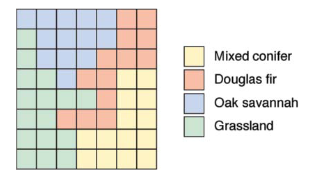
\includegraphics[width=1\linewidth]{images/teori/raster_areal.png}
        \caption{En kategorisk raster hvor hver farve repræsenterer en nominal skala med forskellige arealklasser }
        \label{Subfig: Kategorisk raster}
    \end{subfigure}
    \begin{subfigure} [b]{0.5\textwidth}
        \centering
        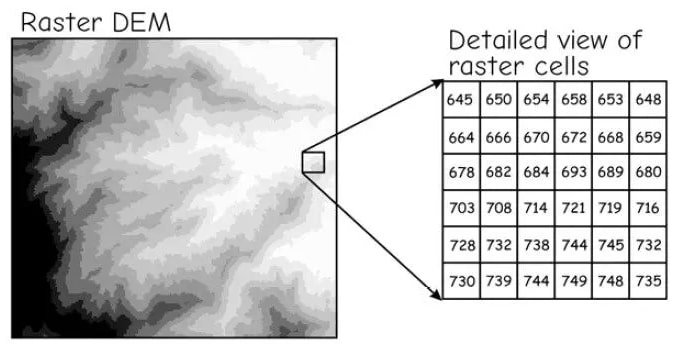
\includegraphics[width=1\linewidth]{images/teori/raster_kontinuert.jpg}
        \caption{En numerisk raster af en Digital Højdemodel (DHM) med en kontinuert skala}
        \label{Subfig: Kontinuer raster}
    \end{subfigure}
    \caption{Eksempel på en kategorisk raster med nominalt data over arealanvendelse og en raster med numeriske kontinuert data fra en højdemodel. Kilde: \cite[s. 67]{longley_geographical_2008} og \cite[s. 66]{bolstad_gis_2022}}
    \label{Figur: Kontinuert og kategorisk raster}
\end{figure}

Rastermodellers struktur gør det muligt at lave rumlig analyse, da der kan udføres aritmetik og logiske udsagn på rasters cellestørrelse og de værdier cellen indholder \citep{bolstad_gis_2022, longley_geographical_2008}. Denne unikke element ved raster datamodellen gør det muligt at regne på tværs af flere raster eller kombinere dem til analysens formål. 


\subsection{Inundation Modellen} \label{Afsnit: Inundation Model}

Til projektet er der blevet anvendt en GIS-baseret stormflods model udarbejdet af \cite{balstrom_kirby_inundation} til at give et bud på hvordan en stormflod vil påvirke et område. \\
Modellen indeholder en række værktøjer, der bruges til at analysere stormfloders påvirkning af et område og kernen i Inundation Modellen er værktøjet \textit{"Create Inundation"} som er en numerisk rastermodel. I figur \ref{Figur: Create Inundation} er flowchartet af modellen. Modellen bruger en række brugerdefineret parametre der består af tre numeriske værdier: InitialSealLevel, SeaLevelIncrement og Number of Iterations. Modellen benytter også en Digital Terræn Model (DTM) og en brugerdefineret linje som kilde for udregningen, benævt Line at Sea \citep{balstrom_kirby_inundation}. 

\begin{figure}[H]
    \centering
    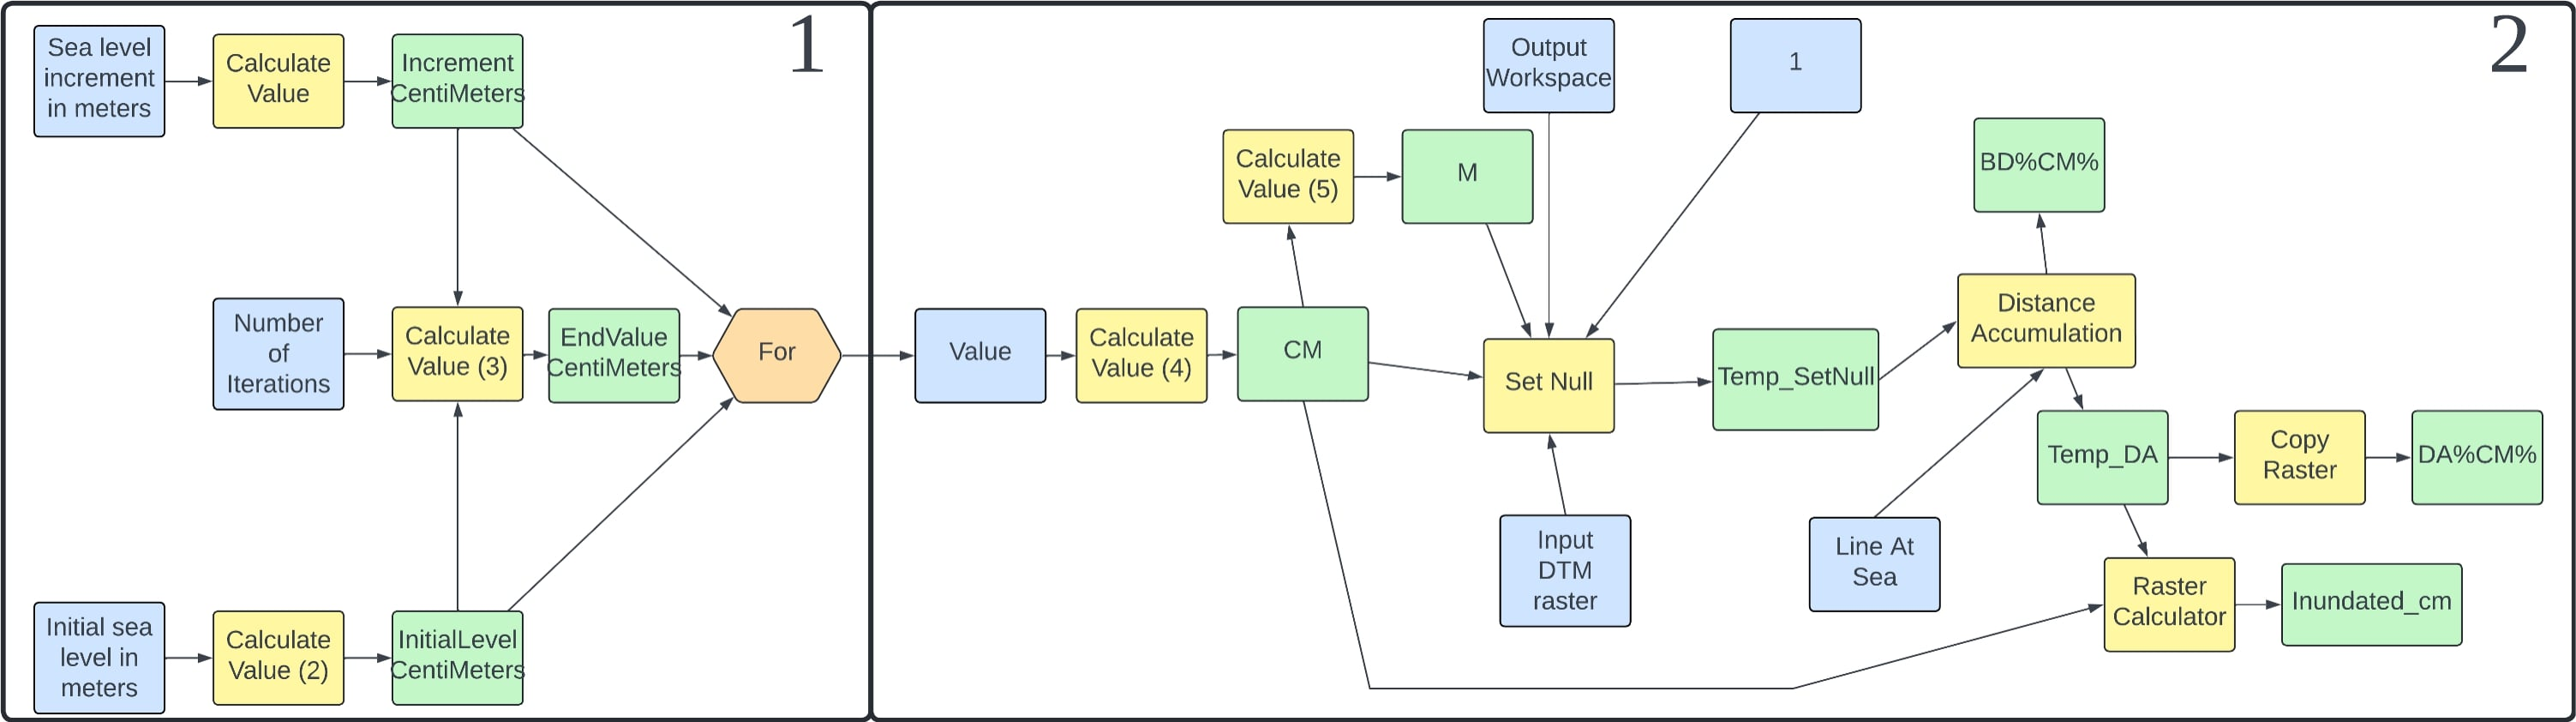
\includegraphics[width=1\linewidth]{images/teori/inundation_model_separated.jpg}
    \caption{Flowchart af Inundation Modellens \textit{"Create Inundation"} værktøj}
    \label{Figur: Create Inundation}
\end{figure}

Modellen er delt op i to komponenter. Den første del er en omregning af brugerens input i meter til centimeter for både stigningsniveauet for hver gang modellen itererer og det begyndende havniveau. Modellen kræver en værdi for hvornår den skal stoppe med at iterere. Denne værdi bliver udregnet ved følgende: $InitialSeaLevel + ((NumberIterations - 1)\times Increment)$. \\

Den anden del af modellen er selve oversvømmelses beregningen gennem terrænet. Det starter med et for-loop der starter med den første værdi (fx 100cm). Denne værdi omregnes tilbage til meter hvorefter modellen eksekverer et tjek (figur \ref{Figur: Create Inundation} "SetNull") på cellerne i DTM. Her tjekkes alle celleværdierne i DTM for om de er \geq den nuværende værdi. Hvis dette hvis-ellers tjek er sandt bliver cellerne tildelt NoData værdien, som indikerer at cellen ikke bliver oversvømmet ved dette oversvømmelsesniveau. Hvis DTM celleværdien er lavere end tjekværdien bliver cellen angivet med et 1, som indikerer at den bliver oversvømmet ved det niveau (figur \ref{Figur: Celler Inundated}).       

\begin{figure}[H]
    \centering
    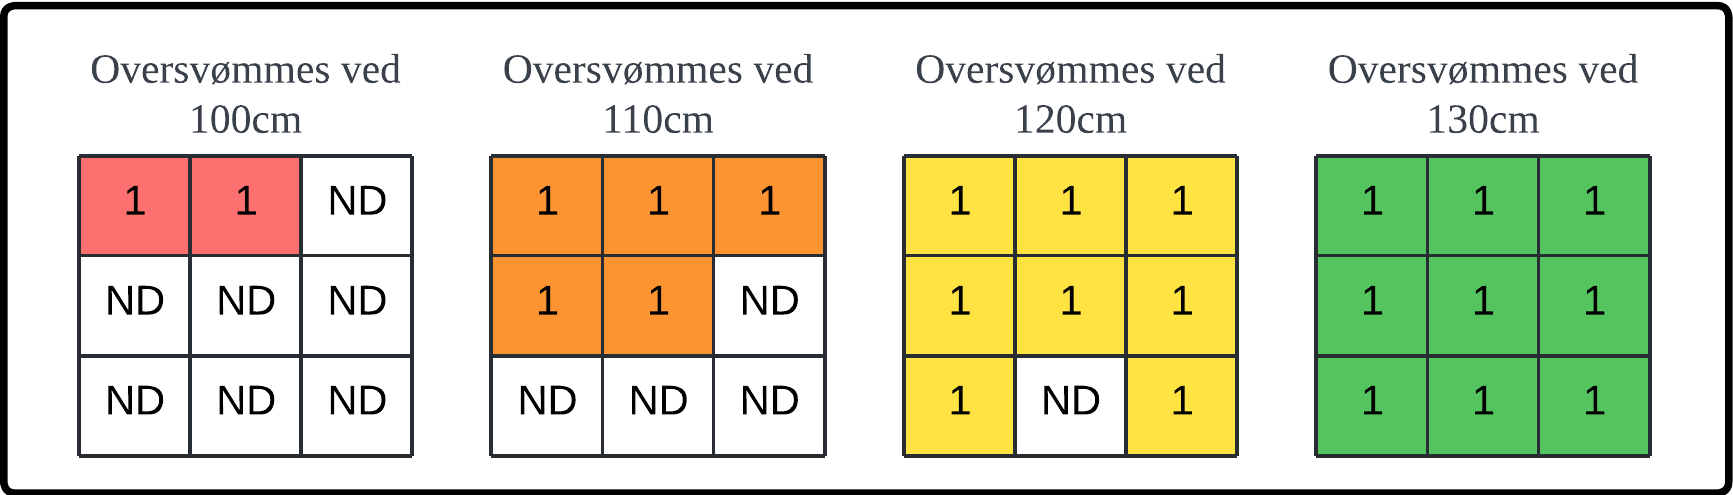
\includegraphics[width=0.7\linewidth]{images/teori/celler_inundated.png}
    \caption{Princippet bag Inundation Modellen gennem raster celler. 1 angiver at cellen oversvømmes ved det pågældende niveau og ND = NoData (celler som ikke bliver oversvømmet).  Egen illustration med inspiration fra \cite{balstrom_kirby_inundation}}
    \label{Figur: Celler Inundated}
\end{figure}

Herefter udføres en Distance Accumulation igennem de celler der bliver oversvømmet ved det bestemte niveau fra en linjekilde. En Distance Accumulation er en analysemetode der beregner den samlede afstand fra en kilde ud igennem et område \citep{esri_how_nodate}. I Inundation modellen bliver Distance Accumulation brugt til at efterligne vandets bevægelse igennem cellerne på samme måde som vandet ville sprede sig under en stormflod. \\ 
Distance Accumulation starter fra linjen \textit{"Line at Sea"} og bevæger sig igennem alle cellerne i terrænet hvor cellen = 1. Hvis cellen er NoData så kan vandet ikke bevæge sig igennem \citep{balstrom_kirby_inundation}. Resultatet af Distance Accumulationen bliver derefter koblet med det oversvømmelsesniveau der bliver itereret over for at give resultatet af modellen.  
